% Options for packages loaded elsewhere
\PassOptionsToPackage{unicode}{hyperref}
\PassOptionsToPackage{hyphens}{url}
\PassOptionsToPackage{dvipsnames,svgnames*,x11names*}{xcolor}
%
\documentclass[
]{article}
\usepackage{lmodern}
\usepackage{amssymb,amsmath}
\usepackage{ifxetex,ifluatex}
\ifnum 0\ifxetex 1\fi\ifluatex 1\fi=0 % if pdftex
  \usepackage[T1]{fontenc}
  \usepackage[utf8]{inputenc}
  \usepackage{textcomp} % provide euro and other symbols
\else % if luatex or xetex
  \usepackage{unicode-math}
  \defaultfontfeatures{Scale=MatchLowercase}
  \defaultfontfeatures[\rmfamily]{Ligatures=TeX,Scale=1}
\fi
% Use upquote if available, for straight quotes in verbatim environments
\IfFileExists{upquote.sty}{\usepackage{upquote}}{}
\IfFileExists{microtype.sty}{% use microtype if available
  \usepackage[]{microtype}
  \UseMicrotypeSet[protrusion]{basicmath} % disable protrusion for tt fonts
}{}
\makeatletter
\@ifundefined{KOMAClassName}{% if non-KOMA class
  \IfFileExists{parskip.sty}{%
    \usepackage{parskip}
  }{% else
    \setlength{\parindent}{0pt}
    \setlength{\parskip}{6pt plus 2pt minus 1pt}}
}{% if KOMA class
  \KOMAoptions{parskip=half}}
\makeatother
\usepackage{xcolor}
\IfFileExists{xurl.sty}{\usepackage{xurl}}{} % add URL line breaks if available
\IfFileExists{bookmark.sty}{\usepackage{bookmark}}{\usepackage{hyperref}}
\hypersetup{
  pdftitle={Homework \#4},
  pdfauthor={Yunting Chiu},
  colorlinks=true,
  linkcolor=Maroon,
  filecolor=Maroon,
  citecolor=Blue,
  urlcolor=blue,
  pdfcreator={LaTeX via pandoc}}
\urlstyle{same} % disable monospaced font for URLs
\usepackage[margin=1in]{geometry}
\usepackage{color}
\usepackage{fancyvrb}
\newcommand{\VerbBar}{|}
\newcommand{\VERB}{\Verb[commandchars=\\\{\}]}
\DefineVerbatimEnvironment{Highlighting}{Verbatim}{commandchars=\\\{\}}
% Add ',fontsize=\small' for more characters per line
\usepackage{framed}
\definecolor{shadecolor}{RGB}{248,248,248}
\newenvironment{Shaded}{\begin{snugshade}}{\end{snugshade}}
\newcommand{\AlertTok}[1]{\textcolor[rgb]{0.94,0.16,0.16}{#1}}
\newcommand{\AnnotationTok}[1]{\textcolor[rgb]{0.56,0.35,0.01}{\textbf{\textit{#1}}}}
\newcommand{\AttributeTok}[1]{\textcolor[rgb]{0.77,0.63,0.00}{#1}}
\newcommand{\BaseNTok}[1]{\textcolor[rgb]{0.00,0.00,0.81}{#1}}
\newcommand{\BuiltInTok}[1]{#1}
\newcommand{\CharTok}[1]{\textcolor[rgb]{0.31,0.60,0.02}{#1}}
\newcommand{\CommentTok}[1]{\textcolor[rgb]{0.56,0.35,0.01}{\textit{#1}}}
\newcommand{\CommentVarTok}[1]{\textcolor[rgb]{0.56,0.35,0.01}{\textbf{\textit{#1}}}}
\newcommand{\ConstantTok}[1]{\textcolor[rgb]{0.00,0.00,0.00}{#1}}
\newcommand{\ControlFlowTok}[1]{\textcolor[rgb]{0.13,0.29,0.53}{\textbf{#1}}}
\newcommand{\DataTypeTok}[1]{\textcolor[rgb]{0.13,0.29,0.53}{#1}}
\newcommand{\DecValTok}[1]{\textcolor[rgb]{0.00,0.00,0.81}{#1}}
\newcommand{\DocumentationTok}[1]{\textcolor[rgb]{0.56,0.35,0.01}{\textbf{\textit{#1}}}}
\newcommand{\ErrorTok}[1]{\textcolor[rgb]{0.64,0.00,0.00}{\textbf{#1}}}
\newcommand{\ExtensionTok}[1]{#1}
\newcommand{\FloatTok}[1]{\textcolor[rgb]{0.00,0.00,0.81}{#1}}
\newcommand{\FunctionTok}[1]{\textcolor[rgb]{0.00,0.00,0.00}{#1}}
\newcommand{\ImportTok}[1]{#1}
\newcommand{\InformationTok}[1]{\textcolor[rgb]{0.56,0.35,0.01}{\textbf{\textit{#1}}}}
\newcommand{\KeywordTok}[1]{\textcolor[rgb]{0.13,0.29,0.53}{\textbf{#1}}}
\newcommand{\NormalTok}[1]{#1}
\newcommand{\OperatorTok}[1]{\textcolor[rgb]{0.81,0.36,0.00}{\textbf{#1}}}
\newcommand{\OtherTok}[1]{\textcolor[rgb]{0.56,0.35,0.01}{#1}}
\newcommand{\PreprocessorTok}[1]{\textcolor[rgb]{0.56,0.35,0.01}{\textit{#1}}}
\newcommand{\RegionMarkerTok}[1]{#1}
\newcommand{\SpecialCharTok}[1]{\textcolor[rgb]{0.00,0.00,0.00}{#1}}
\newcommand{\SpecialStringTok}[1]{\textcolor[rgb]{0.31,0.60,0.02}{#1}}
\newcommand{\StringTok}[1]{\textcolor[rgb]{0.31,0.60,0.02}{#1}}
\newcommand{\VariableTok}[1]{\textcolor[rgb]{0.00,0.00,0.00}{#1}}
\newcommand{\VerbatimStringTok}[1]{\textcolor[rgb]{0.31,0.60,0.02}{#1}}
\newcommand{\WarningTok}[1]{\textcolor[rgb]{0.56,0.35,0.01}{\textbf{\textit{#1}}}}
\usepackage{longtable,booktabs}
% Correct order of tables after \paragraph or \subparagraph
\usepackage{etoolbox}
\makeatletter
\patchcmd\longtable{\par}{\if@noskipsec\mbox{}\fi\par}{}{}
\makeatother
% Allow footnotes in longtable head/foot
\IfFileExists{footnotehyper.sty}{\usepackage{footnotehyper}}{\usepackage{footnote}}
\makesavenoteenv{longtable}
\usepackage{graphicx,grffile}
\makeatletter
\def\maxwidth{\ifdim\Gin@nat@width>\linewidth\linewidth\else\Gin@nat@width\fi}
\def\maxheight{\ifdim\Gin@nat@height>\textheight\textheight\else\Gin@nat@height\fi}
\makeatother
% Scale images if necessary, so that they will not overflow the page
% margins by default, and it is still possible to overwrite the defaults
% using explicit options in \includegraphics[width, height, ...]{}
\setkeys{Gin}{width=\maxwidth,height=\maxheight,keepaspectratio}
% Set default figure placement to htbp
\makeatletter
\def\fps@figure{htbp}
\makeatother
\setlength{\emergencystretch}{3em} % prevent overfull lines
\providecommand{\tightlist}{%
  \setlength{\itemsep}{0pt}\setlength{\parskip}{0pt}}
\setcounter{secnumdepth}{-\maxdimen} % remove section numbering

\title{Homework \#4}
\author{Yunting Chiu}
\date{2021-02-23}

\begin{document}
\maketitle

\begin{enumerate}
\def\labelenumi{\arabic{enumi}.}
\tightlist
\item
  \textbf{(2.17)} An analyst fitted normal error regression model and
  conducted an F test of H0 : \(\beta1\) = 0 versus H1 : \(\beta1\) = 0.
  The P-value of the test was 0.033, and the analyst concluded that
  \(\beta1\) = 0. Was the \(\alpha\) level used by the analyst greater
  than or smaller than 0.033? If the \(\alpha\) level had been 0.01,
  what would have been the appropriate conclusion?
\end{enumerate}

\textbf{An F-statistic greater than the critical value is equivalent to
a p-value less than alpha and both mean that we can reject the null
hypothesis.} With the small p-value 0.033, we have evidence to reject
the null, meaning that \(\alpha\) \textgreater{} 0.033. Plus, 0.033 is
greater than 0.01, so we also can reject the null at \(\alpha\) =
0.01.\\
Reference:
\url{https://stats.stackexchange.com/questions/50727/f-statistic-f-critical-value-and-p-value}

\begin{enumerate}
\def\labelenumi{\arabic{enumi}.}
\setcounter{enumi}{1}
\tightlist
\item
  \textbf{(2.18)} For conducting statistical tests concerning the
  parameter \(\beta1\), why is the t-test more versatile than the
  F-test?
\end{enumerate}

Because t-test has one-sided test(left tail \& right tail), and
two-sided test for \(\beta1\). Conversely, F-test (most notably in
ANOVA) only can detect H0 : \(\beta1\) = 0 v.s. H1 : \(\beta1\) != 0.

\begin{enumerate}
\def\labelenumi{\arabic{enumi}.}
\setcounter{enumi}{2}
\tightlist
\item
  \textbf{(2.19)} When testing H0 : \(\beta1\) = 0 versus H1 :
  \(\beta1\) 6= 0, why is the F-test a one-sided test even though H1
  includes both cases \(\beta1\) \textless{} 0 and \(\beta1\)
  \textgreater{} 0?
\end{enumerate}

The F-stat is always a number that is positive. The large values of
F-stat is support Ha, and the values of F-stat approximate to 1 support
H0. In other words, \(\beta1^2\) \textgreater{} 0, which is the same as
testing whether \(\beta1\) \textgreater{} 0 or \(\beta1\) \textless{} 0,
respectively.

\begin{enumerate}
\def\labelenumi{\arabic{enumi}.}
\setcounter{enumi}{3}
\item
\item
  \textbf{(Continued from HW-2,3)} At a gas station, 180 drivers were
  asked to record the mileage of their cars and the number of miles per
  gallon. The results are summarized in the table.
\end{enumerate}

The sample correlation coefficient is r = -0.17. In the previous
homework, we fit a regression model that described how the number of
miles per gallon depends on the mileage.

\begin{enumerate}
\def\labelenumi{(\alph{enumi})}
\tightlist
\item
  Complete the ANOVA table. Include sums of squares, degrees of freedom,
  mean squares, and the F-statistic.
\end{enumerate}

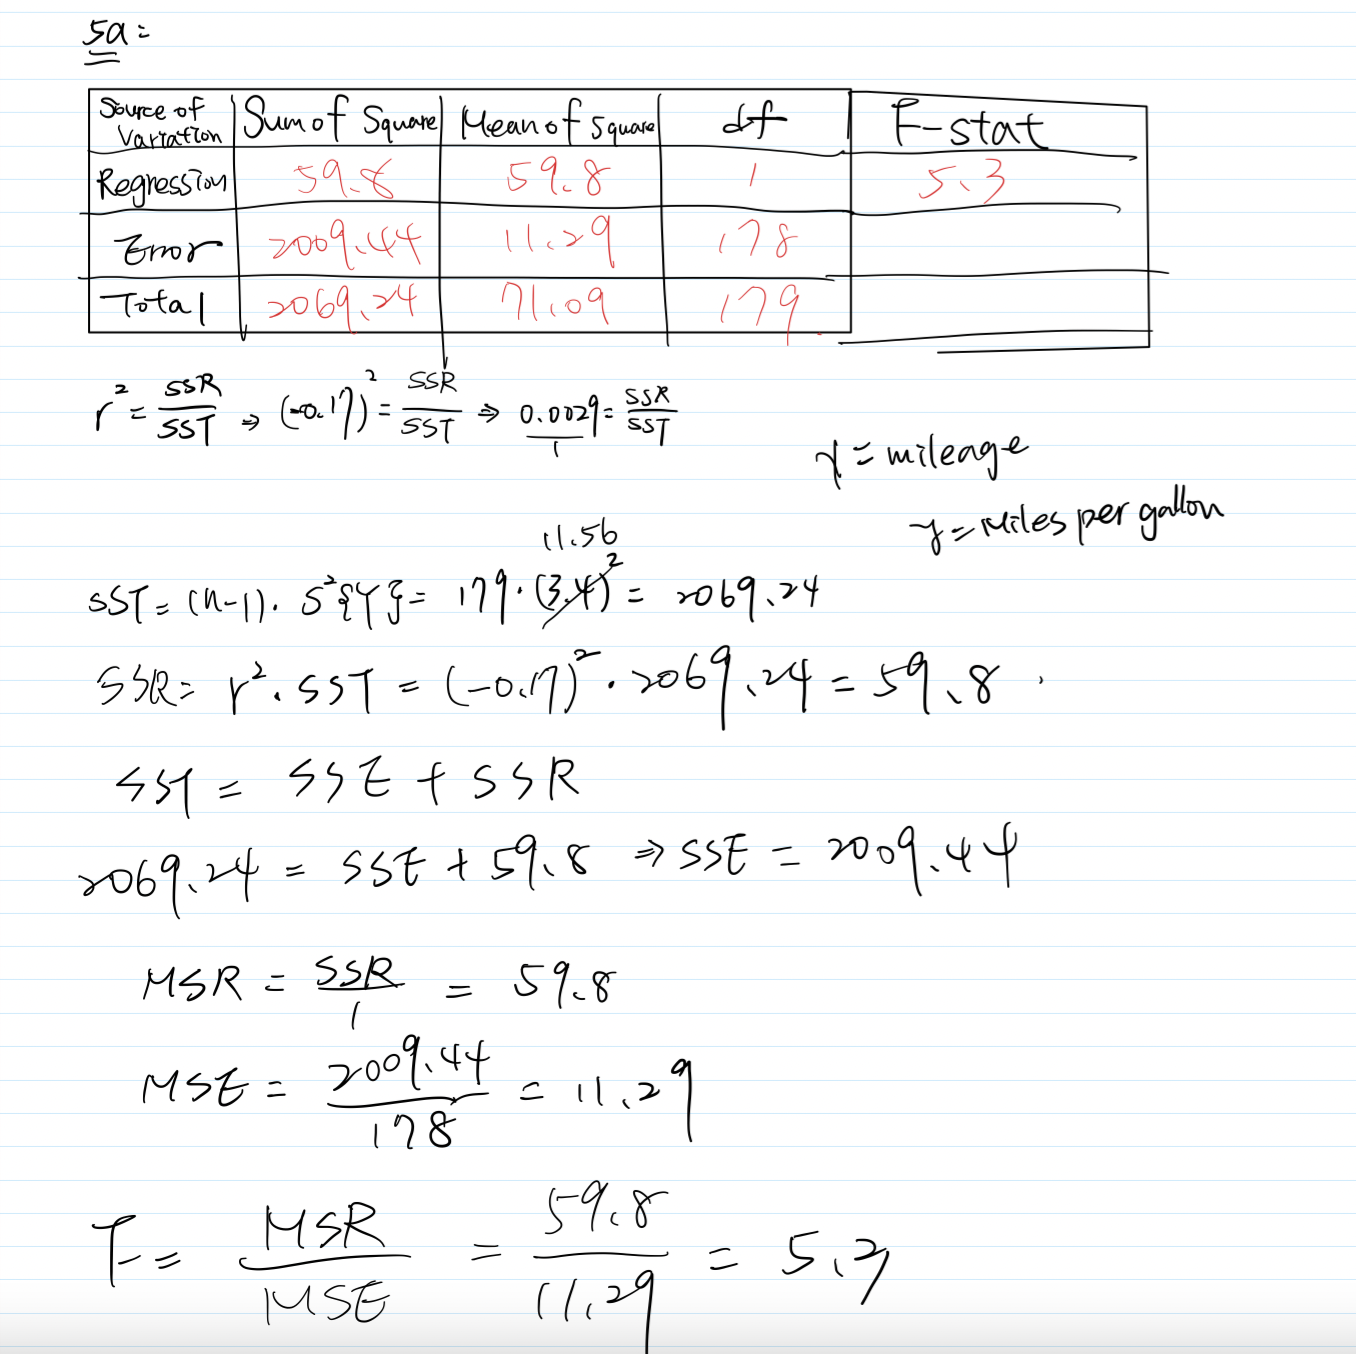
\includegraphics{pics/Screen Shot 2021-02-21 at 4.24.38 PM.png}

\begin{enumerate}
\def\labelenumi{(\alph{enumi})}
\setcounter{enumi}{1}
\tightlist
\item
  What statement can be tested using this F-statistic? Calculate the
  p-value and state a conclusion for this ANOVA F-test.
\end{enumerate}

\begin{itemize}
\tightlist
\item
  F-statistic is 5.3
\item
  Ho: \(\beta1\) = 0 v.s. \(\beta1\) != 0
\item
  According to \href{http://socr.ucla.edu/Applets.dir/F_Table.html}{F
  Distribution Tables}, the F(1, 178) is 5.0239 with \(\alpha\) at
  0.025, F(1, 178) is 6.635 with \(\alpha\) at 0.01. So we can know the
  p-value is between 0.025 to 0.01, meaning that we have evidence
  (\(\alpha\) \textless{} 0.05) to reject the null hypothesis. Also, we
  can conclude that the slope is significant.
\end{itemize}

\begin{enumerate}
\def\labelenumi{(\alph{enumi})}
\setcounter{enumi}{2}
\tightlist
\item
  From your ANOVA table, estimate the standard deviation of responses,
  \(\sigma\) = Std(Yi).\\
\end{enumerate}

The unbiased estimation of standard deviation is 3.36

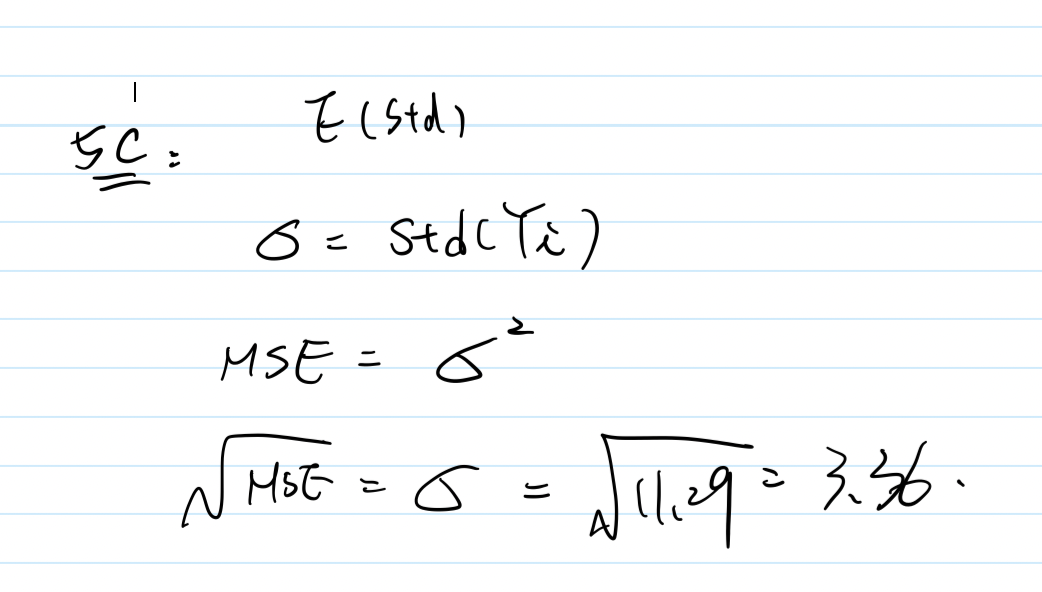
\includegraphics{pics/Screen Shot 2021-02-21 at 8.21.54 PM.png}

\begin{enumerate}
\def\labelenumi{(\alph{enumi})}
\setcounter{enumi}{3}
\tightlist
\item
  Calculate \(R^2\) and comment on the goodness of fit in this
  regression problem.
\end{enumerate}

\(R^2\) = 0.0289 is the straightforward interpretation for the model
because it accounts for the 2.89\% of the total variation in Miles per
gallon explained by Mileage. With a low percentage of \(R^2\), it
doesn't look like fitness in this regression. We might be able to change
another independent variable to fit the model with the dependent
variable Miles per gallon.

\begin{enumerate}
\def\labelenumi{\arabic{enumi}.}
\setcounter{enumi}{5}
\tightlist
\item
  Computer project (2.23, 2.67).\\
  \textbf{Grade point average} (this data set was already used in
  Homework-2,3).
\end{enumerate}

\begin{Shaded}
\begin{Highlighting}[]
\CommentTok{# read the data}
\NormalTok{gpa <-}\StringTok{ }\KeywordTok{read.table}\NormalTok{(}\StringTok{"./data/CH01PR19.txt"}\NormalTok{)}

\NormalTok{reg <-}\StringTok{ }\KeywordTok{lm}\NormalTok{(V1 }\OperatorTok{~}\StringTok{ }\NormalTok{V2, }\DataTypeTok{data =}\NormalTok{ gpa)}
\CommentTok{# call the regression model summary table}
\KeywordTok{summary}\NormalTok{(reg)}
\end{Highlighting}
\end{Shaded}

\begin{verbatim}
## 
## Call:
## lm(formula = V1 ~ V2, data = gpa)
## 
## Residuals:
##      Min       1Q   Median       3Q      Max 
## -2.74004 -0.33827  0.04062  0.44064  1.22737 
## 
## Coefficients:
##             Estimate Std. Error t value Pr(>|t|)    
## (Intercept)  2.11405    0.32089   6.588  1.3e-09 ***
## V2           0.03883    0.01277   3.040  0.00292 ** 
## ---
## Signif. codes:  0 '***' 0.001 '**' 0.01 '*' 0.05 '.' 0.1 ' ' 1
## 
## Residual standard error: 0.6231 on 118 degrees of freedom
## Multiple R-squared:  0.07262,    Adjusted R-squared:  0.06476 
## F-statistic:  9.24 on 1 and 118 DF,  p-value: 0.002917
\end{verbatim}

\begin{enumerate}
\def\labelenumi{(\alph{enumi})}
\tightlist
\item
  Set up the ANOVA table. Use it to answer questions (b-e).
\end{enumerate}

\begin{Shaded}
\begin{Highlighting}[]
\KeywordTok{anova}\NormalTok{(reg)}
\end{Highlighting}
\end{Shaded}

\begin{verbatim}
## Analysis of Variance Table
## 
## Response: V1
##            Df Sum Sq Mean Sq F value   Pr(>F)   
## V2          1  3.588  3.5878  9.2402 0.002917 **
## Residuals 118 45.818  0.3883                    
## ---
## Signif. codes:  0 '***' 0.001 '**' 0.01 '*' 0.05 '.' 0.1 ' ' 1
\end{verbatim}

\begin{enumerate}
\def\labelenumi{(\alph{enumi})}
\setcounter{enumi}{1}
\tightlist
\item
  (Stat-615 only) What is estimated by MSR in your ANOVA table? by MSE?
  Under what conditions do MSR and MSE estimate the same quantity?\\
\end{enumerate}

\begin{longtable}[]{@{}llll@{}}
\toprule
Source & Sum of square & degrees of freedom & Mean of
square\tabularnewline
\midrule
\endhead
Regression & 3.588 & 1 & 3.5878\tabularnewline
Error & 45.818 & 118 & 0.3883\tabularnewline
Total & 49.406 & 119 &\tabularnewline
\bottomrule
\end{longtable}

If \(\beta1\) = 0, meaning that MSR and MSE estimate the same quantity.
In this situation, X and Y does not have a linear association.

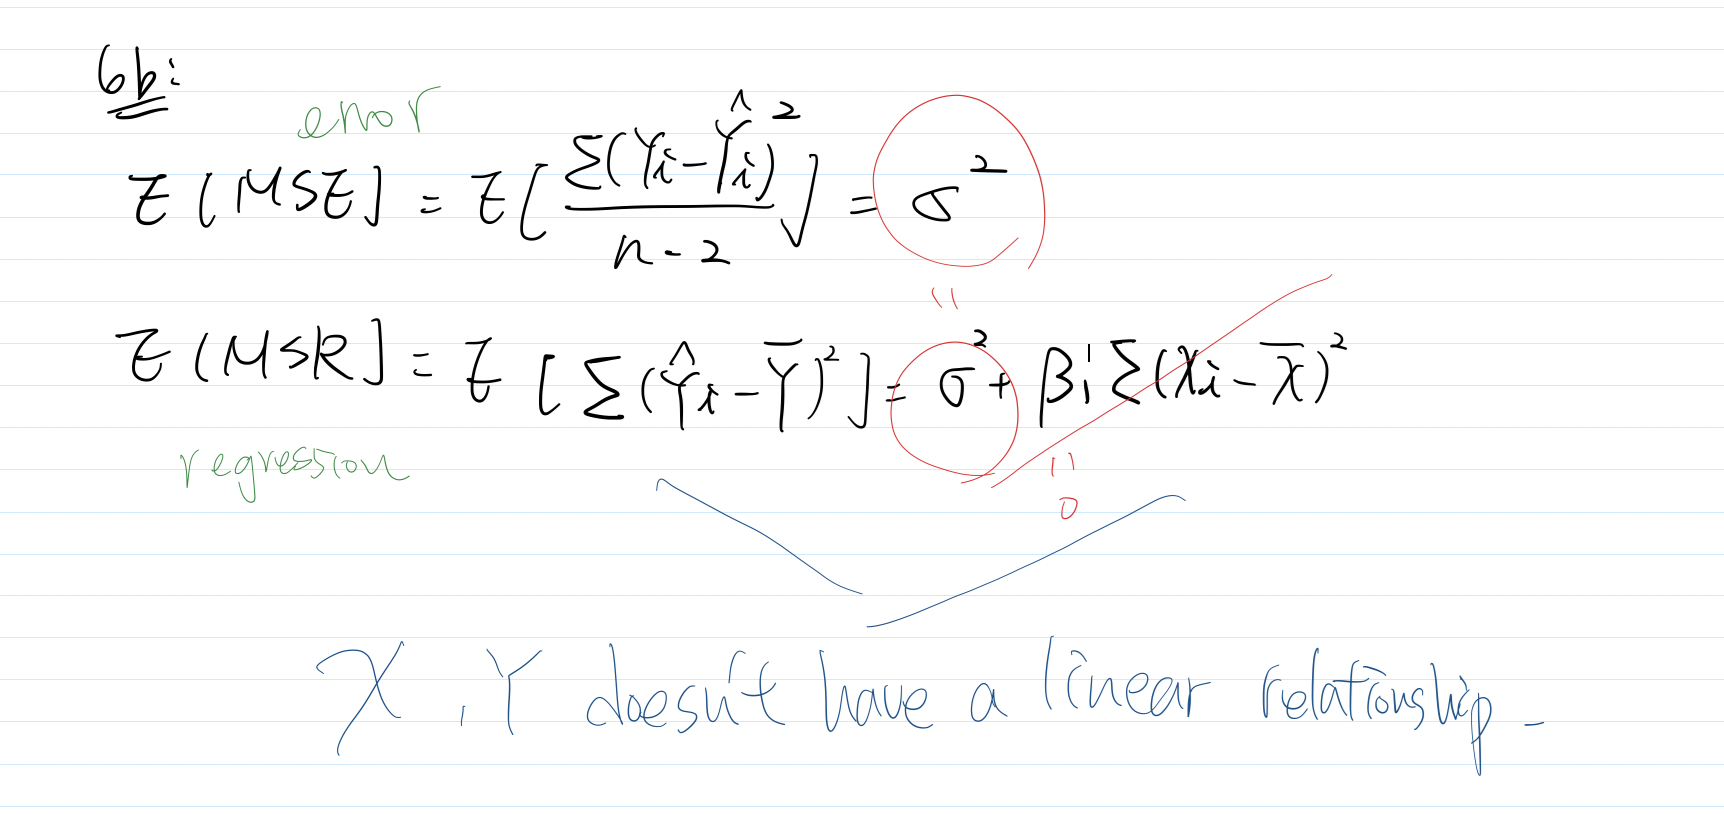
\includegraphics{pics/Screen Shot 2021-02-21 at 3.36.08 PM.png}

Reference:
\url{https://stats.stackexchange.com/questions/175437/mse-and-msr-in-regression-question}

\begin{enumerate}
\def\labelenumi{(\alph{enumi})}
\setcounter{enumi}{2}
\tightlist
\item
  Conduct an F-test of whether or not \(\beta1\) = 0. Control the
  \(\alpha\) level at 0.01. State the alternative and your conclusion
\end{enumerate}

Based on the ANOVA table above, the F-test is 9.2402, and the p-value
falls into significant level between 0.001 to 0.01. We can conclude the
null hypothesis can be rejected at level 0.001 \textless= \(\alpha\)
\textless= 0.01 in favor of the alternative hypothesis.

\begin{enumerate}
\def\labelenumi{(\alph{enumi})}
\setcounter{enumi}{3}
\tightlist
\item
  How much does the variation of Y reduce when X is introduced into the
  regression model? What is the relative reduction?
\end{enumerate}

SST = 49.406, SSE = 45.818, SSR = 3.588. The coefficient of
determination is 7 \%. It means that 7 \% of total variation of GPA
score is explained by the ACT score.

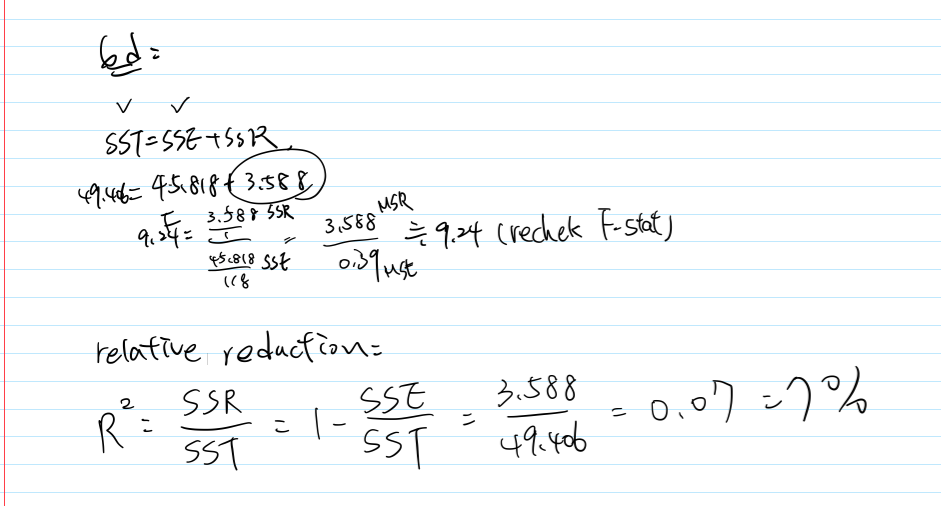
\includegraphics{pics/Screen Shot 2021-02-19 at 1.51.21 PM.png}

\begin{enumerate}
\def\labelenumi{(\alph{enumi})}
\setcounter{enumi}{4}
\tightlist
\item
  Obtain the sample correlation coefficient and attach the appropriate
  sign to it, positive or negative.
\end{enumerate}

Firstly, \(\beta1\) is 0.03883, which is positive slope so the
correlation coefficient is a positive number. Thus, the sample
correlation coefficient is 0.26.

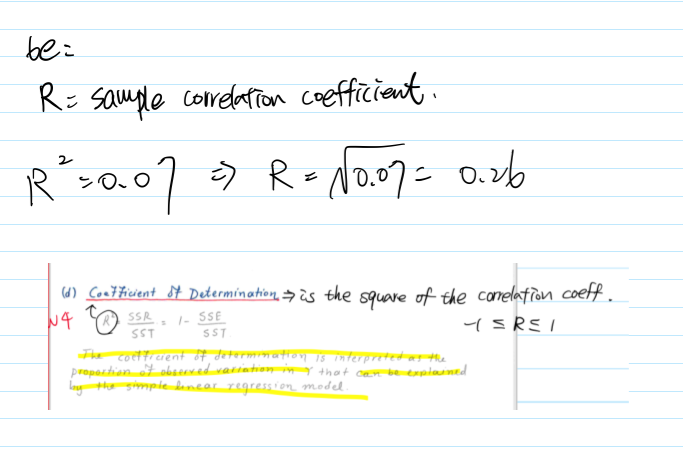
\includegraphics{pics/Screen Shot 2021-02-19 at 1.59.41 PM.png}

\begin{enumerate}
\def\labelenumi{(\alph{enumi})}
\setcounter{enumi}{5}
\tightlist
\item
  (leftover from the last homework) On the same graph, plot
\end{enumerate}

• the data\\
• the least squares regression line for ACT scores\\
• the 95 percent confidence band for the true regression line for ACT
scores between 20 and 30\\

\begin{Shaded}
\begin{Highlighting}[]
\CommentTok{# confidence band for the entire population regression line}
\KeywordTok{attach}\NormalTok{(gpa)}
\NormalTok{n =}\StringTok{ }\KeywordTok{length}\NormalTok{(V2) }\CommentTok{#sample sizes}
\NormalTok{e =}\StringTok{ }\NormalTok{reg}\OperatorTok{$}\NormalTok{residuals }\CommentTok{# residuals}
\NormalTok{s =}\StringTok{ }\KeywordTok{sqrt}\NormalTok{(}\KeywordTok{sum}\NormalTok{(e}\OperatorTok{^}\DecValTok{2}\NormalTok{)}\OperatorTok{/}\NormalTok{(n}\DecValTok{-2}\NormalTok{)) }\CommentTok{# estimated standard deviation = root MSE}
\NormalTok{s}
\end{Highlighting}
\end{Shaded}

\begin{verbatim}
## [1] 0.623125
\end{verbatim}

\begin{Shaded}
\begin{Highlighting}[]
\NormalTok{W =}\StringTok{ }\KeywordTok{sqrt}\NormalTok{(}\DecValTok{2}\OperatorTok{*}\KeywordTok{qf}\NormalTok{(}\FloatTok{0.95}\NormalTok{,}\DecValTok{2}\NormalTok{,n}\DecValTok{-2}\NormalTok{))  }\CommentTok{# quantity of F-distribution}
\NormalTok{W}
\end{Highlighting}
\end{Shaded}

\begin{verbatim}
## [1] 2.479149
\end{verbatim}

\begin{Shaded}
\begin{Highlighting}[]
\NormalTok{Yhat =}\StringTok{ }\KeywordTok{fitted.values}\NormalTok{(reg) }\CommentTok{# Yhat = b0 + b1x = predict(reg)}
\NormalTok{Sxx =}\StringTok{ }\NormalTok{(n}\DecValTok{-1}\NormalTok{)}\OperatorTok{*}\KeywordTok{var}\NormalTok{(V2) }\CommentTok{# sum of the squares of the difference between each x and its mean}

\NormalTok{margin =}\StringTok{ }\NormalTok{W}\OperatorTok{*}\NormalTok{s}\OperatorTok{*}\KeywordTok{sqrt}\NormalTok{(}\DecValTok{1}\OperatorTok{/}\NormalTok{n }\OperatorTok{+}\StringTok{ }\NormalTok{(V2 }\OperatorTok{-}\StringTok{ }\KeywordTok{mean}\NormalTok{(V2))}\OperatorTok{^}\DecValTok{2}\OperatorTok{/}\NormalTok{Sxx) }
\NormalTok{upper.band =}\StringTok{ }\NormalTok{Yhat }\OperatorTok{+}\StringTok{ }\NormalTok{margin }\CommentTok{# 95% upper }
\NormalTok{lower.band =}\StringTok{ }\NormalTok{Yhat }\OperatorTok{-}\StringTok{ }\NormalTok{margin }\CommentTok{# 95% lower}

\KeywordTok{plot}\NormalTok{(V2, V1, }\DataTypeTok{xlab =} \StringTok{"ACT Score"}\NormalTok{, }\DataTypeTok{ylab =} \StringTok{"Y = fresh Year GPA"}\NormalTok{, }\DataTypeTok{xlim =} \KeywordTok{c}\NormalTok{(}\DecValTok{20}\NormalTok{,}\DecValTok{30}\NormalTok{))}
\KeywordTok{abline}\NormalTok{(reg,}\DataTypeTok{col=}\StringTok{"red"}\NormalTok{)}
\KeywordTok{lines}\NormalTok{(V2 ,upper.band,}\DataTypeTok{col=}\StringTok{"blue"}\NormalTok{)}
\KeywordTok{lines}\NormalTok{(V2 ,lower.band,}\DataTypeTok{col=}\StringTok{"blue"}\NormalTok{)}
\end{Highlighting}
\end{Shaded}

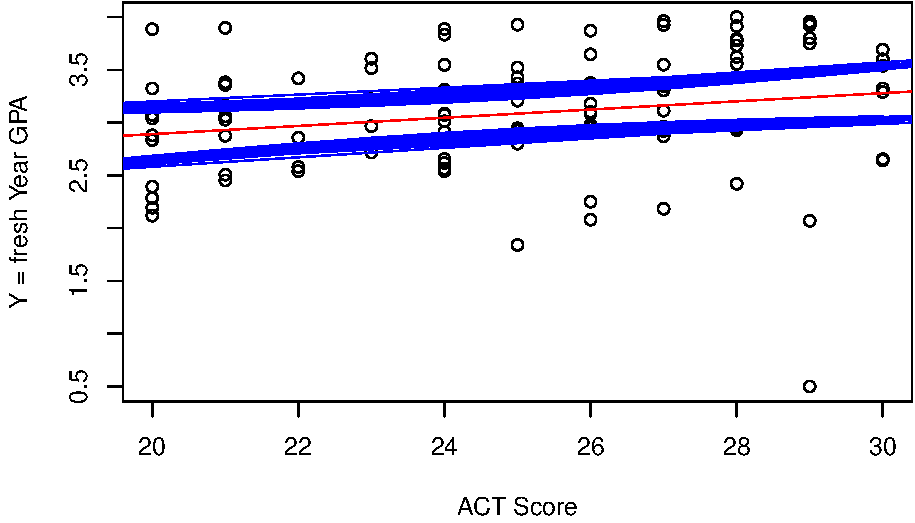
\includegraphics{Yunting_HW4_files/figure-latex/unnamed-chunk-3-1.pdf}

\end{document}
